
\documentclass[12pt,onecolumn]{article}
\usepackage[brazilian]{babel}
\usepackage[utf8]{inputenc}
\usepackage{graphicx}
\usepackage{caption}
\usepackage{subcaption}
\usepackage{float}
\usepackage{hyperref}

\begin{document}

\title{Apostila de WordPress}
\author{Cara A \\ Cara B}
\maketitle

\section{Sobre o WordPress}
	O wordpress é dahora.

\section{Instalando}
	O \href{http://codex.wordpress.org/Installing_WordPress}{guia oficial} do 
	WordPress cobre todos os casos comuns, então nada melhor que utilizar a documentação oficial.
	
	TODO: tecer alguns comentários sobre a instalação, mesmo assim.
	Lorem ipsum dolor sit amet, consectetur adipiscing elit. Pellentesque tincidunt quam ac augue posuere in malesuada urna pellentesque. Donec odio libero, tristique ut dictum ut, convallis in odio. Aliquam id imperdiet dui. Suspendisse tristique tortor in enim rhoncus placerat. Curabitur imperdiet tortor ac diam cursus gravida. Aliquam consectetur fermentum ligula, non consequat tortor porta non. Quisque commodo vestibulum consequat. Nunc aliquet nisi vitae felis sollicitudin ultrices. Vestibulum congue facilisis nunc, nec dignissim ipsum mattis adipiscing. 

\section{Postando Lixo}

	\subsection{Autorização}
		É importante notar que o WordPress possui um controle de acesso, logo 
		somente pessoas autorizadas podem criar novos posts.
		
		Para tal, precisamos então realizar o login.
		\begin{figure}[H]
			\begin{subfigure}{.4\textwidth}
				\centering
				
\includegraphics{login1.png}
				\caption{Link para a página de login}
			\end{subfigure}
			\begin{subfigure}{.4\textwidth}
				\centering
				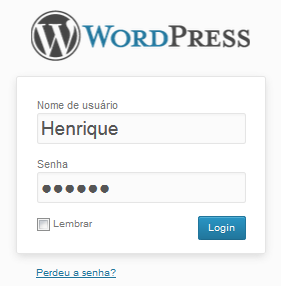
\includegraphics{login2.png}
				\caption{Digitando usuário e senha}
			\end{subfigure}
			\caption{Processo de login}
		\end{figure}
	
	\subsection{Criando um post}
		TODO: é simples que só imagens bastam
		\begin{figure}[H]
			\centering
			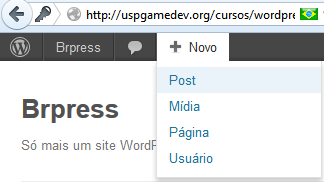
\includegraphics{post1.png}
			\caption{Usando a barra do WordPress}
		\end{figure}
		\begin{figure}[H]
			\centering
			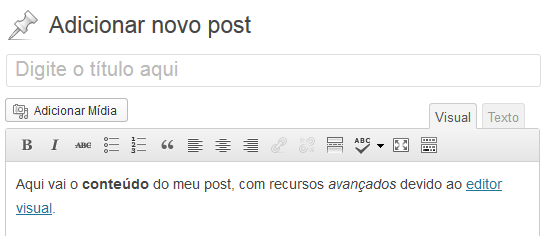
\includegraphics{post2.png}
			\caption{Usando o editor visual}
		\end{figure}
		\begin{figure}[H]
			\centering
			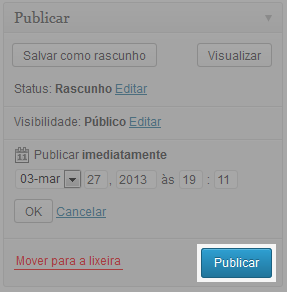
\includegraphics{post3.png}
			\caption{Publicando}
		\end{figure}
		
\end{document}
